\documentclass{article}
\usepackage[spanish]{babel}
\usepackage[utf8]{inputenc}
\usepackage{amsmath}
\usepackage{amssymb}
\usepackage{verbatim}
\usepackage{graphicx}
\usepackage{listings}
\usepackage{fullpage}
\usepackage{color}
\usepackage{fancyvrb}
\usepackage{hyperref}

\definecolor{mygreen}{rgb}{0,0.6,0}
\definecolor{mygray}{rgb}{0.5,0.5,0.5}
\definecolor{mymauve}{rgb}{0.58,0,0.82}

\lstset{ %
	backgroundcolor=\color{white},   % choose the background color; you must add \usepackage{color} or \usepackage{xcolor}
	basicstyle=\footnotesize,        % the size of the fonts that are used for the code
	breakatwhitespace=false,         % sets if automatic breaks should only happen at whitespace
	breaklines=true,                 % sets automatic line breaking
	captionpos=b,                    % sets the caption-position to bottom
	commentstyle=\color{mygreen},    % comment style
	frame=single,                    % adds a frame around the code
	keepspaces=true,                 % keeps spaces in text, useful for keeping indentation of code (possibly needs columns=flexible)
	numbers=left,                    % where to put the line-numbers; possible values are (none, left, right)
	numbersep=5pt,                   % how far the line-numbers are from the code
	numberstyle=\tiny\color{mygray}, % the style that is used for the line-numbers
	rulecolor=\color{black},         % if not set, the frame-color may be changed on line-breaks within not-black text (e.g. comments (green here))
	showspaces=false,                % show spaces everywhere adding particular underscores; it overrides 'showstringspaces'
	showstringspaces=false,          % underline spaces within strings only
	showtabs=false,                  % show tabs within strings adding particular underscores
	stepnumber=1,                    % the step between two line-numbers. If it's 1, each line will be numbered
	stringstyle=\color{mymauve},     % string literal style
	tabsize=4,                       
	title=\lstname                   % show the filename of files included with \lstinputlisting; also try caption instead of title
}


\author{José Luis Cánovas Sánchez}
\title{ARQUITECTURAS DE REDES AVANZADAS\\PRÁCTICA 1\\ 2015/2016}
\date{}
\begin{document}
\maketitle

\begin{abstract}
	En este informe se redacta el desarrollo e instrucciones para llevar a cabo las configuraciones de varios servicios descritos durante el desarrollo de la asignatura de Servicios Telemáticos. Tenemos varios servicios que para funcionar dependen de otros, de modo que se podría intentar ir creando cada cosa según se necesite, o bien suponer que el servicio del que se depende es totalmente funcional y, de este modo, ir configurando cada servicio completamente, y una vez todos los servicios de los que se depende están configurados, poner en marcha el subsistema que forman. En este artículo seguiremos este segundo método, de modo que veremos una evolución del sistema: configuración, puesta en marcha, estudio de los servicios y protocolos utilizados.
\end{abstract}

\tableofcontents
\section{Introducción}
El sistema a desarrollar será el del dominio st.um, el cual consta en principio de dos equipos o \textit{hosts}, cada uno con un papel bien definido: el primer host será el servidor, con FQDN (\textit{fully qualified domain name})  servidor.st.um, y actuará como servidor de servicios de DNS, NTP, web (HTTP/HTTPS) y correo (SMTP/POP); por otro lado tenemos al host cliente, con FQDN cliente.st.um, que hará uso de servidor.st.um para comprobar que funcionan correctamente.\par

\begin{center} 
	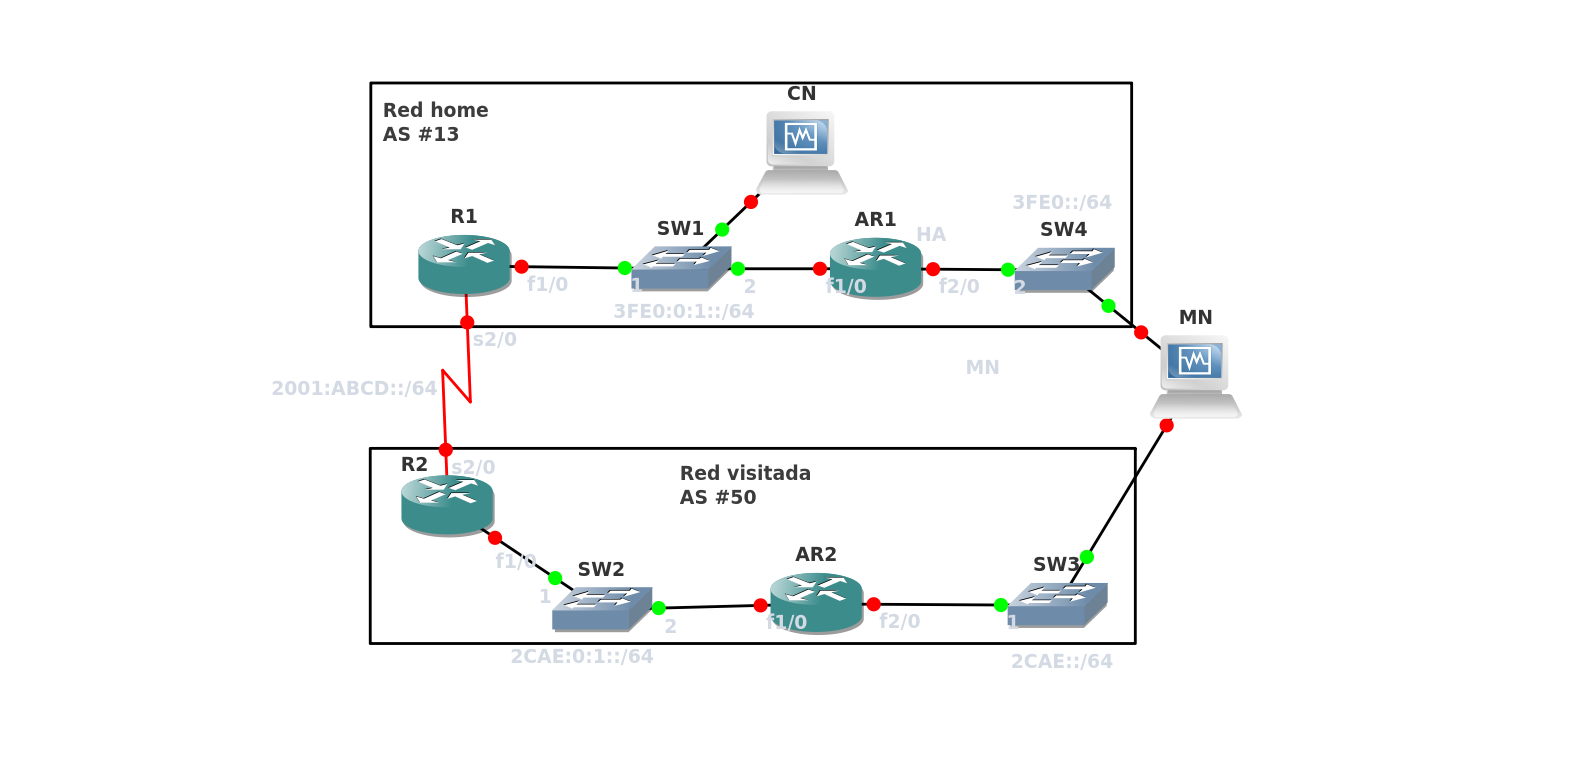
\includegraphics[scale=0.5]{images/topologyInic.png}
\end{center}

Parece conveniente hacer una introducción sencilla de cada protocolo de modo que cuando lleguemos a la configuración, tengamos una visión general del camino que estamos tomando.\par

\end{document}
